\documentclass[11pt,a4paper]{article}

\usepackage{graphicx,tabularx}      
\usepackage{float}
\usepackage[T1]{fontenc}
\usepackage[utf8]{inputenc}
\usepackage[a4paper,margin=2.2cm]{geometry}
\usepackage{array}
\usepackage{longtable}
\usepackage{tabularx}
\usepackage{booktabs}
\usepackage{graphicx}
\usepackage{xcolor}
\usepackage{caption}
\usepackage{enumitem}
\usepackage{pdflscape}
\usepackage[hidelinks]{hyperref}

\captionsetup{font=small,labelfont=bf}
\setlength{\parskip}{4pt}
\setlength{\parindent}{0pt}
\renewcommand{\arraystretch}{1.15}

\newcolumntype{L}[1]{>{\raggedright\arraybackslash}p{#1}}

\title{\textbf{Securing the Festo Smart Factory Lab}\\[2pt]}
\author{Aleksander Kłap \& Lourdes Gaurisse}
\date{June 15, 2026}

\begin{document}

\maketitle
\pagebreak
\tableofcontents
\listoffigures
\pagebreak

\section{List of Attachments}
The following materials are provided as attachments to this
report.
\begin{table}[H]
\centering
\setlength{\tabcolsep}{6pt}
\begin{tabular}{L{1.4cm} L{4.5cm} L{9cm}}
\toprule
\textbf{Ref} & \textbf{Attachment} & \textbf{Description} \\
\midrule
    A1 & Festo Plant AS-IS Network Diagram & See chapter 4.2. Attached for better
    visibility. \\

    A2 & TO-BE Architecture Zones \& Conduits Diagram & See chapter 8.1.
    Attached for better visibility. \\

    A3 & TO-BE Network Implementation Architecture & See chapter 8.2. Attached
    for better visibility. \\

    A4 & In-practice weak passord break-in evidence & See chapter 5.4. \\

    A5 & Hands-on Attack on Hardware evidence & See chapter 6.5. \\

\bottomrule
\end{tabular}
    \caption{List of Attachments}\label{attachments}
\end{table}

\section{Introduction \& Scope}\label{intro}
This report assesses and redesigns the cybersecurity posture of the 
Fontys Festo Smart Factory Lab 4.0. The factory is functionally operational
but was not designed against state-of-the-art OT security
principles.
\vspace{1em}

The work follows four phases: describe the current (AS-IS) state, perform a
threat and risk analysis, specify security requirements, and design a
secure-by-design (TO-BE) architecture including supporting hardware
recommendation and procedures to follow. The goal is to protect availability,
integrity, and confidentiality while keeping the lab operational.

\vspace{1em}
\textbf{Scope.} The project covers the OT/ICS network of the
lab with the six manufacturing stations The work is to understand and
analyse the factory as it currently runs, assess the
security risks, and design a new architecture that is secure
and meets the required security measures.
\vspace{1em}

\textbf{Standards.} The redesign is based on the standards
and principles required by the assignment: 
\begin{itemize}
    \item IEC~62443
    \item ISO/IEC~27001
    \item NIS2 Directive
    \item Defense-in-Depth principle, 
    \item Least Privilege \& Zero Trust (industrial interpretation)
\end{itemize}

\pagebreak

% SECTION FESTO Description
\section{Festo Factory Description}\label{festodesc}
The Festo CPLab is a modular production line representing a
modern Industry~4.0 plant. It consists of seven cells:
\vspace{0.5em}
\begin{itemize}[nosep]
  \item Station 0 --- Robot Arm: Universal Robots UR3e pick-and-place cobot with a Turck RFID reader.
  \item Station 1 --- Conveyor Belt: transport between stations.
  \item Station 2 --- Ball Sorting / Dispense: sorting and dispensing, with remote I/O and a power monitor.
  \item Station 3 --- Camera Inspection: SensoPart vision sensor for quality inspection.
  \item Station 4 --- Magazine: part storage and a Festo CPX cloud-connected valve/IO terminal.
  \item Station 5 --- Muscle Press: pneumatic press.
  \item Station 6 --- Oven: curing/heating, with a Festo CPX controller and power monitor.
\end{itemize}

\vspace{0.5em}
The line runs as an order-driven manufacturing process. A production order
enters through the MES, which is linked to a webshop, and the MES schedules the
job and releases it to the line. Each workpiece is identified by RFID and
tracked as it moves between stations on the conveyor. The robot arm handles
pick-and-place, and the workpiece passes through the stations for sorting and
dispensing, pressing, oven curing, and camera inspection before storage in the
magazine. Station status and results are reported back to the MES, which tracks
each order through to completion. The hardware, network, and protocols behind
this flow are detailed in the following sections.

\section{AS-IS Architecture}\label{asisarch}
This section documents the Festo Plant factory in its current operational
setup. \\

\subsection{Asset Inventory}\label{assetinventory}
{\scriptsize
\setlength{\tabcolsep}{3pt}

\paragraph{Network Infrastructure}
\begin{longtable}{L{2cm} L{2.1cm} L{2.1cm} L{2.6cm} L{2.4cm} L{4cm}}
\toprule
\textbf{Asset} & \textbf{Model} & \textbf{IP} & \textbf{MAC} & \textbf{Protocols} & \textbf{Function} \\
\midrule \endhead
    MES PC & SIMATIC-PC & 172.21.0.90 & 4c:d7:17:90:73:a2 & OPC
    UA, NTP, HTTP, HTTPS & MES, MES database, NTP server \\

    MQTT device & Festo & 172.21.0.210 & 00:0E:F0:7C:A3:C0 &
    MQTT & MQTT device publishing telemetry data to MES \\

    Router & TP-Link router & 172.21.0.200 &
    20:23:51:41:a2:88 & UDP & Router \\
\bottomrule
\end{longtable}

\paragraph{Station 0 --- Robot Arm Station (172.21.1.x/18)}
\begin{longtable}{L{2cm} L{2.1cm} L{2.1cm} L{2.6cm} L{2.4cm} L{4cm}}
\toprule
\textbf{Asset} & \textbf{Model} & \textbf{IP} & \textbf{MAC} & \textbf{Protocols} & \textbf{Function} \\
\midrule \endhead
    Switch S0 & Siemens SCALANCE XB008 & unmanaged & unmanaged &
    Ethernet & Station 0 network distribution \\

    PLC  - TODO\\

    HMI  - TODO\\

    Robot Arm Controller & UR3e & TODO ip & TODO mac & Profinet & Pick \& place robot arm control \\ 

    RFID Reader & Turck TBEN-S2-2RFID-4DXP & 172.21.1.20 &
    00:07:46:aa:07:cc & PROFINET & RFID identification of transport trays \\
\bottomrule
\end{longtable}


\paragraph{Station 1 --- Conveyor Belt (172.21.1.x)}
\begin{longtable}{L{2cm} L{2.1cm} L{2.1cm} L{2.6cm} L{2.4cm} L{4cm}}
\toprule
\textbf{Asset} & \textbf{Model} & \textbf{IP} & \textbf{MAC} & \textbf{Protocols} & \textbf{Function} \\
\midrule \endhead
    Switch S1 & Siemens SCALANCE XB008 & unmanaged & unmanaged & Ethernet &
    Station 1 distribution \\

    HMI S1 & Siemens MTP700 Unified Comfort & 172.21.1.10 & 30:13:89:35:da:a8 &
    PROFINET & Operator panel \\

    PLC S1 & Siemens CPU 1512SP F-1 PN / V3.0.3 & 172.21.1.1 &
    30:B8:51:32:D3:E7 & PROFINET, HTTP, OPC-UA, S7comm & Process control S1 \\

    PC Cobot-ML & unknown & 172.21.1.90 & 08:bf:b8:f1:25:e3 & OPC-UA, HTTP &
    Image Processing \\
\bottomrule
\end{longtable}

\paragraph{Station 2 --- Ball Sorting / Dispense (172.21.2.x)}
\begin{longtable}{L{2cm} L{2.1cm} L{2.1cm} L{2.6cm} L{2.4cm} L{4cm}}
\toprule
\textbf{Asset} & \textbf{Model / Firmware} & \textbf{IP} & \textbf{MAC} & \textbf{Protocols} & \textbf{Function} \\
\midrule \endhead
    Switch S2 & Siemens SCALANCE XB008 & unmanaged & unmanaged & Ethernet &
    Station 2 distribution \\

    PLC S2 & Siemens CPU 1512SP F-1 PN / V3.0.3 & 172.21.2.1 & 30:b8:51:33:7e:c7 & PROFINET, HTTP, OPC-UA, S7comm & Process control S2 \\

    HMI S2 & Siemens MTP700 Unified Comfort & 172.21.2.10 & 30:13:89:35:d8:af &
    PROFINET, S7comm+, NTP & Operator panel \\

    FESTO COntroller - TODO \\

    Power Monitor S2 & Siemens & 172.21.2.61 & 10:DF:FC:17:DC:72 & TODO & Power
    consumption monitoring \\

    IO Device & Siemens ET200SP IM155-6PN/2 HF / V4.2.4 & 172.21.2.100 &
    4c:e7:05:4b:46:4b & PROFINET IO & Remote IO module - ball dispenser control \\
\bottomrule
\end{longtable}

\paragraph{Station 3 --- Camera Inspection (172.21.3.x)}
\begin{longtable}{L{2cm} L{2.1cm} L{2.1cm} L{2.6cm} L{2.4cm} L{4cm}}
\toprule
\textbf{Asset} & \textbf{Model / Firmware} & \textbf{IP} & \textbf{MAC} & \textbf{Protocols} & \textbf{Function} \\
\midrule \endhead
    Switch S3 & Siemens SCALANCE XB008 & unmanaged & unmanaged & Ethernet &
    Station 3 distribution \\

    PLC S3 & Siemens CPU 1512SP F-1 PN / V3.0.3 & 172.21.3.1 & 30:b8:51:32:d3:9b &
    PROFINET, HTTP, OPC-UA, S7comm & Process control S3 \\

    HMI S3 & Siemens MTP700 Unified Comfort & 172.21.3.10 & 30:13:89:2c:e9:c5 &
    PROFINET & Operator panel \\

    Camera & SensoPart & 172.21.3.50 & 00:19:6F:0D:A3:72 & HTTP & Monitoring ball distribution on tray \\

\bottomrule
\end{longtable}

\paragraph{Station 4 --- Magazine (172.21.4.x)}
\begin{longtable}{L{2cm} L{2.1cm} L{2.1cm} L{2.6cm} L{2.4cm} L{4cm}}
\toprule
\textbf{Asset} & \textbf{Model / Firmware} & \textbf{IP} & \textbf{MAC} & \textbf{Protocols} & \textbf{Function} \\
\midrule \endhead
    Switch S4 & Siemens SCALANCE XB008 & unmanaged & unmanaged & Ethernet &
    Station 4 distribution \\

    PLC S4 & Siemens CPU 1512SP F-1 PN / V3.0.3 & 172.21.4.1 & 30:b8:51:33:7e:24 &
    PROFINET, HTTP, OPC-UA, S7comm & Process control S4 \\

    HMI S4 & Siemens MTP700 Unified Comfort & 172.21.4.10 & 30:13:89:35:D9:EF &
    PROFINET & Operator panel \\

    CPX Terminal & Festo CPX (197330) & TODO & TODO & TODO & Agreggate Festo Controllers monitoring data \\
\bottomrule
\end{longtable}

\paragraph{Station 5 --- Muscle Press (172.21.5.x)}
\begin{longtable}{L{2cm} L{2.1cm} L{2.1cm} L{2.6cm} L{2.4cm} L{4cm}}
\toprule
\textbf{Asset} & \textbf{Model / Firmware} & \textbf{IP} & \textbf{MAC} & \textbf{Protocols} & \textbf{Function} \\
\midrule \endhead
    Switch S5 & Siemens SCALANCE XB008 & unmanaged & unmanaged & Ethernet &
    Station 5 distribution \\

    PLC S5 & Siemens CPU 1512SP F-1 PN / V3.0.3 & 172.21.5.1 & 30:b8:51:33:7e:62 &
    PROFINET, HTTP, OPC-UA, S7comm & Process control S5 \\

    HMI S5 & Siemens MTP700 Unified Comfort & 172.21.5.10 & 30:13:89:36:6A:EE &
    PROFINET & Operator panel \\

\bottomrule
\end{longtable}

\paragraph{Station 6 --- Oven (172.21.6.x)}
\begin{longtable}{L{2cm} L{2.1cm} L{2.1cm} L{2.6cm} L{2.4cm} L{4cm}}
\toprule
\textbf{Asset} & \textbf{Model / Firmware} & \textbf{IP} & \textbf{MAC} & \textbf{Protocols} & \textbf{Function} \\
\midrule \endhead
HMI S6 & Siemens MTP700 Unified Comfort & 172.21.6.10 & 30:13:89:35:d9:c7 & PROFINET & Operator panel \\

Switch S6 & Siemens SCALANCE XB008 & unmanaged & unmanaged & Ethernet & Station 6 distribution \\

PLC S6 & Siemens CPU 1512SP F-1 PN / V3.0.3 & 172.21.6.1 & 30:B8:51:32:D4:5F & PROFINET, HTTP, OPC-UA, S7comm & Process control S6 \\

FESTO Controller - TODO\\

Power Monitor S6 & TODO & 172.21.6.61 & 10:DF:FC:17:DC:6C & TODO & Power consumption monitoring \\
\bottomrule
\end{longtable}
} % end scriptsize

\subsection{Network Diagram}\label{asisnetdiagram}
Through physical inspection of the Festo plant, nmap host
discovery, and Wireshark traffic captures, we mapped the
current network architecture. The result is shown in the
diagram below. \vspace{0.5em}\\
For better visibility, this diagram is attached separatly to the report.

\begin{figure}[H]
    \centering
    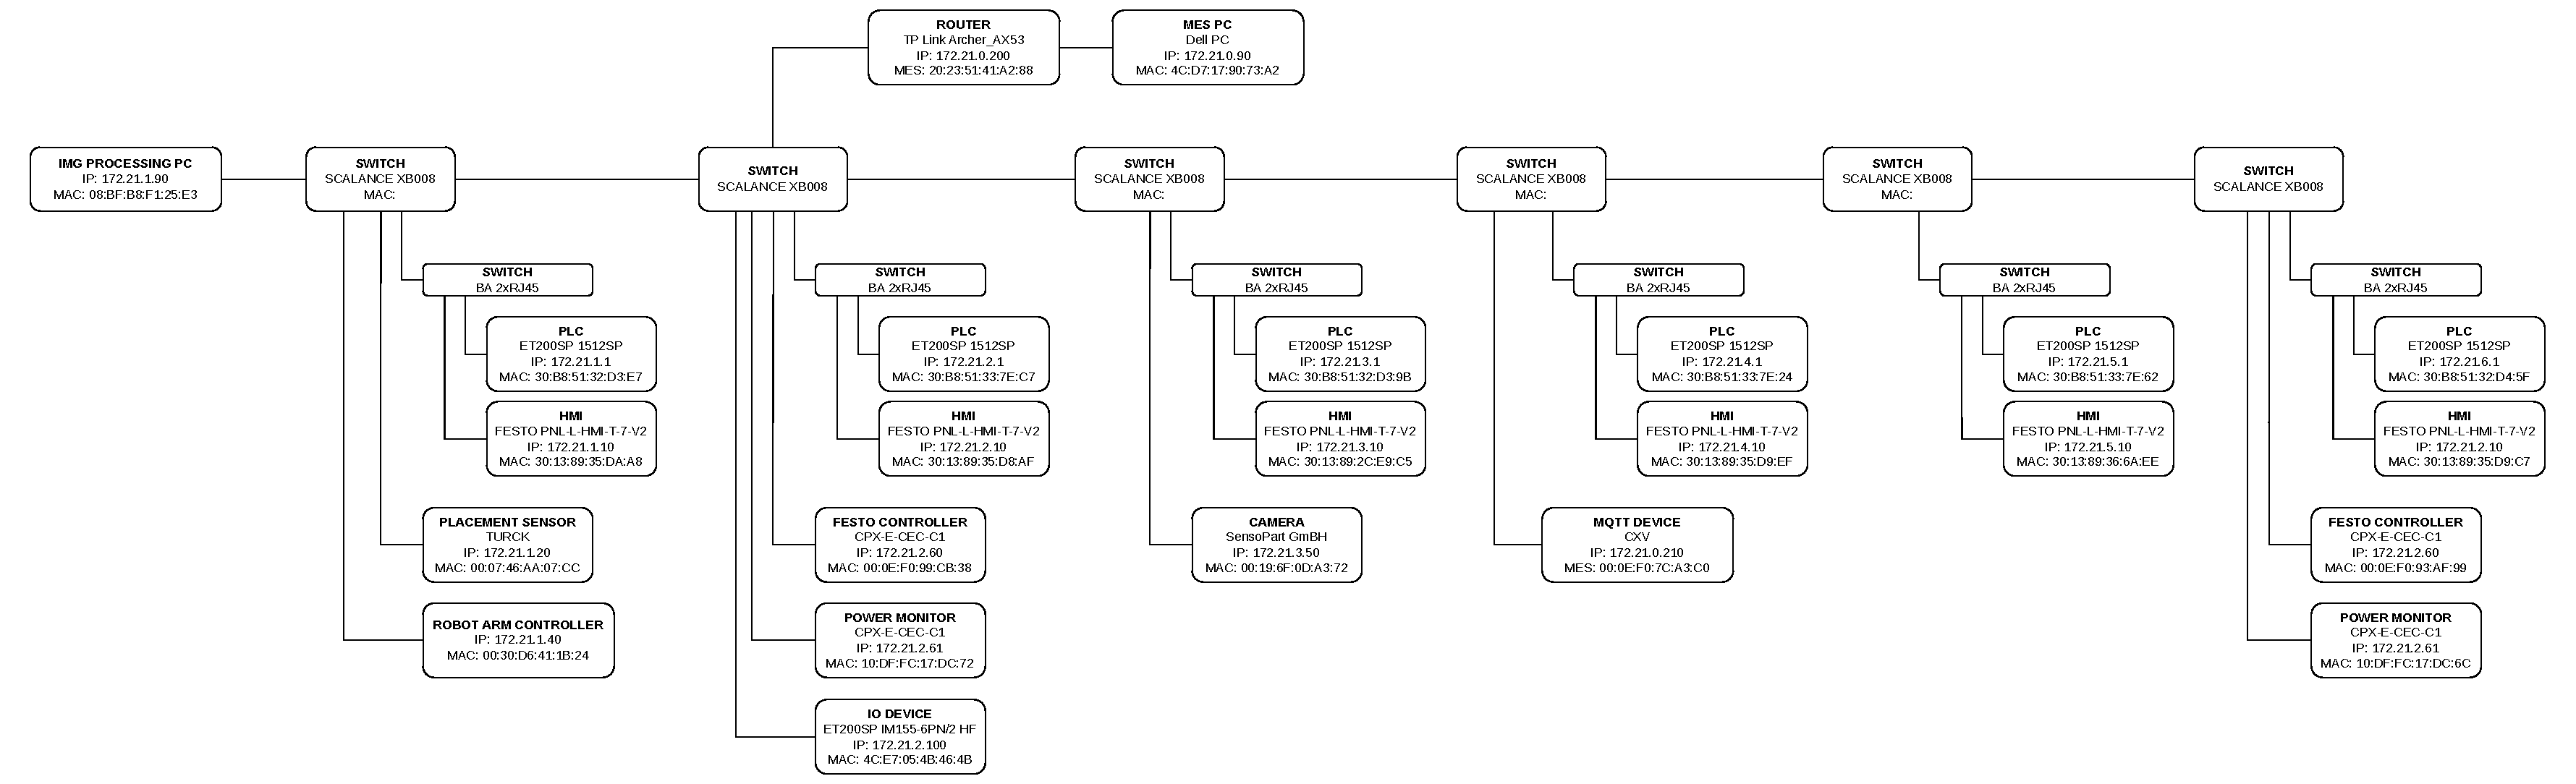
\includegraphics[width=1\textwidth]{img/festo_plant_network_architecture_diagram.pdf}
    \caption{AS-IS Network Diagram}
\end{figure}

%% SUBSection Communication Mapping
\subsection{Communication Mapping}\label{protocolmatrix}
{\small
\setlength{\tabcolsep}{4pt}
\begin{longtable}{L{2.6cm} L{2.0cm} L{1.8cm} L{1.8cm} L{3.4cm} L{3.2cm}}
\toprule
\textbf{Source} & \textbf{Destination} & \textbf{Protocol} & \textbf{Port} & \textbf{Direction} & \textbf{Purpose} \\
\midrule \endhead
    MES & PLC & OPC-UA & TCP 4840 & MES(OPC-UA Client) to
    PLC(OPC-UA Server) & Read/write process data \\ 

    HMI / PLC & MES & NTP & UDP 123 &
    Clients(HMI/PLC) to MES(NTP Server) & Time sync (MES is NTP server) \\

    Internet & MES & HTTPS & TCP 443 & Internet to MES &
    Webshop orders \\ 

    Cobot-ML PC & Camera & HTTP & TCP 80 & Cobot-ML to
    Camera & Fetch inspection image from Camera server \\ 

    Cobot-ML PC & PLC & OPC-UA & TCP 4840 & Cobot-ML to PLC & 
    Process data - based on image processing \\

    PLC & IO Device & PROFINET &
    L2 / 34964 & PLC to IO & Cyclic I/O exchange \\ 

    Festo Controller & CPX-IOT (CVX) & MQTT & TCP 1883 &
    Controller to CVX & Publish aggregated data \\ 

    RFID Reader & PLC & PROFINET & L2 / 34964 & Reader to PLC &
    RFID identification \\ 

    PLC & Robot Arm & PROFINET & L2 /
    34964 & PLC to Robot & Motion commands / status \\ 

    HMI & PLC & S7comm+ & TCP 102 & HMI to PLC & Read/write
    tags for panel \\ 

    MES PC & PLC & S7comm-plus & TCP 102 & MES to PLC & PLC programming \\ 

    MES PC & HMI & S7comm-plus & TCP 102 & MES to HMI & HMI
    programming/config \\ 

    Power Monitor & Festo Controller & Modbus & TCP 502
    & Monitor to Controller & Power consumption data \\
\bottomrule
\end{longtable}
}

\pagebreak

\section{AS-IS Architecture Security Analysis}\label{asissecanalysis}

\subsection{Security Weaknesses}\label{secweaknesses}
The overall security posture is critical. There is no real barrier
between the IT systems, engineering PCs, visitor devices, and the live control
equipment. One compromised device can reach every PLC and HMI. The findings
below are rated by how easy they are to exploit and their impact on
availability, safety, and integrity.

\begin{longtable}{L{1.3cm} L{1.8cm} L{12.0cm}}
\caption{Security weaknesses summary}\\
\toprule
\textbf{ID} & \textbf{Severity} & \textbf{Finding} \\
\midrule \endhead
F-01 & CRITICAL & Fully flat /18 network --- no zone or conduit separation \\
F-02 & CRITICAL & PLCs directly reachable from all hosts --- no access control \\
F-03 & CRITICAL & MES PC has unrestricted protocol access to all OT devices \\
F-04 & CRITICAL & Unregistered device actively programming PLCs via S7comm \\
F-05 & HIGH & PLC web servers expose HTTP (plaintext) on the OT subnet \\
F-06 & HIGH & TP-Link AP on OT subnet --- potential wireless attack surface \\
F-07 & HIGH & Visitor/unvetted laptop (Kyan\_laptop) on live OT network \\
F-08 & HIGH & gebruik-tt8ke80 runs VMware with unknown VM roles on OT subnet \\
F-09 & MEDIUM & PROFINET carries no authentication --- DCP allows rename/reconfigure \\
F-10 & LOW & NTP provided only by MES PC --- single point of failure \\
\bottomrule
\end{longtable}

\subsection{Security Weaknesses Findings}\label{secfindings}
\newcommand{\finding}[4]{%
\par\smallskip\noindent\textbf{#1}\\[2pt]
\begin{tabularx}{\linewidth}{@{}L{2.7cm} X@{}}
\textit{Observation} & #2 \\
\textit{Impact} & #3 \\
\end{tabularx}\par}

\finding{F-01 --- Fully flat /18 network (IEC 62443-1-1; 3-3 SR 5.1/5.2; ISO 27001 A.8.22; NIS2 Art.~21)}
{All 21+ live hosts share 172.21.0.0/18 with no VLAN, routed boundary, or firewall between device classes. PLCs, HMIs, MES, engineering PCs, visitor laptops, and infrastructure share one broadcast domain.}
{Any compromised host has Layer~3 reachability to every PLC, HMI, and sensor. Lateral movement from an infected laptop to all six PLCs requires no further exploitation.}

\finding{F-02 --- Unrestricted PLC access (IEC 62443-3-3 SR 1.1/1.2/5.1)}
{All S7-1500 PLCs expose HTTP/80, OPC-UA/4840, and S7comm/102 to the whole subnet, with no authentication observed at the network layer.}
{Any host can connect to any PLC's S7comm port, read/write process data, up/download program blocks, or force a CPU STOP without credentials. All six stations are simultaneously vulnerable.}

\finding{F-03 --- No MES/OT separation (IEC 62443-2-1; 3-3 SR 5.2; ISO 27001 A.8.22)}
{festo-mes-pc communicates directly with PLC~S2 via HTTP (alarm polling), OPC-UA (process data), and NTP --- unmediated, with no DMZ or proxy.}
{Compromise of the Windows MES PC gives an attacker a trusted, persistent connection to PLC~S2's control interface; a malformed PLC response could also exploit the MES software.}

\finding{F-04 --- Unregistered device programming PLCs (IEC 62443-2-1; ISO 27001 A.8.1/A.8.19; Zero Trust)}
{172.21.0.156 maintained a persistent, high-volume S7comm session to PLC~S2 across all captures and appears in no inventory; behaviour is consistent with TIA Portal in active programming mode.}
{An unidentified device with S7comm write access to a live PLC is a rogue-programmer scenario: it can alter logic, inject faults, or cause unsafe states on Station~2 with no audit trail.}

\finding{F-05 --- PLC HTTP web servers in plaintext (IEC 62443-3-3 SR 1.3; Defense-in-Depth)}
{PLC~S2 serves HTTP/80; the MES issues unauthenticated GET requests to the alarm table about every 3~s. No TLS/HTTPS observed; the same web server exists on all PLCs.}
{Alarm and diagnostic data travels in plaintext and can be intercepted or spoofed by any subnet host, which can also reach the diagnostic web interface without authentication.}

\finding{F-06 --- TP-Link access point on OT subnet (NIS2 Art.~21; IEC 62443-2-1; Defense-in-Depth)}
{172.21.0.200 was identified via UPnP SSDP as a TP-Link device running MiniUPnPd, broadcasting on UDP/20002.}
{A wireless interface bridged to the OT subnet removes the physical perimeter; consumer firmware has a poor patch record, and MiniUPnPd is an internet-facing port-forwarding daemon that may expose OT services.}

\finding{F-07 --- Visitor/unvetted laptop on OT network (NIS2 Art.~21(2)(h); IEC 62443-2-1; Zero Trust)}
{Kyan\_laptop (172.21.0.179) was identified by DCP as SIMATIC-PC family (PROFINET drivers installed) and admitted to the OT subnet without restriction.}
{A personal/student laptop is more likely to carry malware or be used on untrusted networks; once on the OT subnet it has the same PLC access as any device.}

\finding{F-08 --- VMware host with unknown VM roles (ISO 27001 A.8.1; IEC 62443-2-1; Defense-in-Depth)}
{gebruik-tt8ke80 presents a physical NIC and a VMware vNIC at the same IP; hosted VM roles and OS are unknown, and bridged VMs inherit OT subnet membership.}
{An internet-connected or unpatched VM provides a path from an untrusted environment to OT; hypervisor flaws can enable VM escape to a host with physical-layer OT access.}

\paragraph{Medium / Low findings.}
\begin{itemize}[nosep]
  \item \textbf{F-9:} Restrict PROFINET (L2, EtherType 0x8892) to known switch ports via VLAN/port security; disable DCP Set on production devices where supported.
  \item \textbf{F-10:} Add a secondary NTP source and authenticate NTP (NTS or keys).
\end{itemize}


\subsection{Standards Compliance Status}\label{standardsstatus}
\begin{longtable}{L{3.6cm} L{4.6cm} L{3.8cm} L{2.6cm}}
\caption{AS-IS standards compliance summary}\\
\toprule
\textbf{Standard / Requirement} & \textbf{Requirement summary} & \textbf{Current status} & \textbf{Findings} \\
\midrule \endhead
IEC 62443-1-1 Zone \& Conduit & Define zones; control conduits & NOT MET --- single flat zone & F-01, F-02, F-03 \\
IEC 62443-2-1 CSMS & Asset inventory, risk, access, change control & PARTIAL --- incomplete inventory & F-04, F-09, F-15 \\
IEC 62443-3-3 SR 5.1/5.2 & Segmentation; zone boundary protection & NOT MET & F-01, F-02, F-03 \\
IEC 62443-3-3 SR 1.1/1.2 & User/device authentication & NOT MET --- no auth on S7comm, HTTP, PROFINET & F-02, F-05, F-06, F-11 \\
ISO/IEC 27001 A.8.1 & Complete, maintained asset register & PARTIAL --- 6+ devices absent & F-04, F-09, F-15 \\
ISO/IEC 27001 A.8.22 & Segregate services and users & NOT MET & F-01 \\
NIS2 Art.~21 & Segmentation, access control, asset mgmt & NOT MET & F-01--F-09 \\
NIS2 Art.~21(2)(e) & Supply-chain risk management & NOT MET --- unverified firmware & F-10, F-13 \\
Defense-in-Depth & Multiple independent layers & NOT MET --- single perimeter & F-01--F-04 \\
Least Privilege & Minimum necessary access & NOT MET --- unrestricted subnet access & F-02, F-03, F-06 \\
Zero Trust & No implicit trust from location & NOT MET --- trust by /18 membership & F-02, F-04, F-08 \\
\bottomrule
\end{longtable}

\subsection{In-practice weak password break-in}\label{weakpass}
Beyond the findings based on traffic and network analysis, we
obtained one practical finding: a weak system password. On the
MES PC Windows login screen, after entering a wrong password,
Windows displayed a hint stating the password was no longer the
previous value. Based on this hint, it took only two tries to
guess the current password, and we were able to log in to the
MES PC, which students are not supposed to access.

Furthermore, going through the HTTP servers of the Festo plant
nodes, we found that every element requiring authentication
accepted the same password revealed by the Windows hint. This
allowed us to log in to many hardware elements of the factory
with high privileges, including user management, stopping
services, and changing configuration. 

Proof of this access is attached to the report.

\section{Threat \& Risk Analysis}\label{threatrisk}
The analysis follows IEC~62443 principles and a simplified STRIDE model adapted
for ICS. Industrial systems are sensitive because compromise can directly
affect physical processes, safety, and production continuity, not just data.

\subsection{Attacker Profiles}
\begin{itemize}[nosep]
  \item \textbf{External attacker:} motivated by financial gain, disruption, or opportunistic exploitation; relies on phishing, misconfigured remote access, or known vulnerabilities.
  \item \textbf{Insider:} a user with legitimate access (operator, engineer, contractor); can bypass perimeter controls and poses the highest risk for silent tampering.
  \item \textbf{Student / opportunistic actor:} low sophistication but high local/physical access; responsible for accidental misconfiguration or simple exploitation of weak segmentation.
\end{itemize}

\subsection{Threat Scenarios}
\begin{itemize}[nosep]
  \item \textbf{PLC manipulation:} modifying control logic or setpoints, causing unsafe actuator behaviour or bypassed interlocks, usually via a compromised engineering workstation or insider access.
  \item \textbf{Denial of Service:} flooding network segments or exploiting protocol weaknesses to disrupt PLC/SCADA/HMI communication.
  \item \textbf{Unauthorized device access:} a rogue device introduced physically or via misconfiguration scans, impersonates trusted nodes, or interacts with PLC services.
  \item \textbf{Malware via Engineering PC:} a compromised engineering workstation pivots into PLC networks, extracts logic, or deploys malicious changes --- one of the most critical ICS vectors.
  \item \textbf{Data manipulation via MES/Webshop:} altering production orders, parameters, or scheduling, leading to incorrect batches and downstream disruption.
\end{itemize}

\subsection{Threat Table}
{\small
\setlength{\tabcolsep}{4pt}
\begin{longtable}{L{2.2cm} L{2.6cm} L{2.2cm} L{2.8cm} L{1.4cm} L{2.2cm}}
\caption{ICS threat analysis matrix (IEC 62443-based)}\\
\toprule
\textbf{Asset} & \textbf{Threat} & \textbf{Attacker} & \textbf{STRIDE} & \textbf{Impact} & \textbf{Example} \\
\midrule \endhead
Engineering PC & Malware infection & External / Student & Info.\ disclosure, Tampering & Critical & Phishing leads to PLC compromise \\
Engineering PC & Unauthorized access & Insider & Elevation of privilege & Critical & Engineer account reused/misused \\
PLCs & Logic manipulation & External / Insider & Tampering, EoP & High & Modified logic alters actuators \\
PLCs & Command injection & Student / External & Spoofing & High & Fake control commands \\
SCADA/HMI & Session hijacking & External & Spoofing & High & Operator session impersonated \\
Network segments & Traffic flooding & External & Denial of service & High & Broadcast storm disrupts PLCs \\
PLC network & Config exfiltration & External & Info.\ disclosure & High & PLC logic downloaded \\
MES system & Production manipulation & External / Insider & Tampering & High & Batch parameters altered \\
SCADA/HMI & Denial of service & External & Denial of service & Med--High & Operator loses visibility \\
Webshop/API & Data modification & External & Tampering, Info.\ disclosure & Med--High & Order data changed \\
Network switches & Rogue device & Student / Insider & Spoofing & Medium & Unauthorized laptop joins VLAN \\
\bottomrule
\end{longtable}
}

\subsection{Risk Matrix}\label{riskmatrix}
Likelihood and impact are scored 1--4; risk score is their product.

{\small
\setlength{\tabcolsep}{4pt}
\begin{longtable}{L{4.0cm} L{1.8cm} L{6.0cm} L{1.4cm} L{1.6cm}}
\caption{ICS threat risk assessment}\\
\toprule
\textbf{Threat} & \textbf{Likelihood} & \textbf{Impact (safety / production / education)} & \textbf{Score} & \textbf{Priority} \\
\midrule \endhead
Engineering PC malware infection & High (3) & Critical (4): full control-layer
    compromise, persistent access & 12 & Critical \\

    PLC logic manipulation & Medium (2) & Critical (4): unsafe actuators,
    shutdown, learning disruption & 8 & High \\

    Unauthorized engineering access (insider) & Medium (2) & Critical (4):
    silent logic changes, safety bypass & 8 & High \\

    SCADA/HMI denial of service & Medium (2) & High (3): loss of visibility,
    interruption & 6 & Medium \\

    Network flooding / traffic storm & Medium (2) & High (3): loss of PLC
    comms, downtime & 6 & Medium \\

    MES production manipulation & Medium (2) & High (3): incorrect runs,
    financial/operational impact & 6 & Medium \\

    PLC config/data exfiltration & Medium (2) & High (3): IP loss, enables
    future attacks & 6 & Medium \\

    Rogue device in network & Medium (2) & Medium (2): recon, lateral movement
    & 4 & Medium \\

    Webshop/API data manipulation & Medium (2) & Medium (2): incorrect orders,
    indirect issues & 4 & Medium \\

    PLC command spoofing & Low (1) & High (3): incorrect actions, physical
    instability & 3 & Low \\

    Session hijacking (SCADA) & Low (1) & High (3): stealth manipulation, loss
    of trust & 3 & Low \\
\bottomrule
\end{longtable}
}
\subsection{Hands-on Attack on Hardware}\label{profinetattack}
To better understand the nature of a possible attack, we
executed a denial-of-service attack on the I/O device: a
PROFINET DCP station name change attack. PROFINET DCP
(Discovery and Configuration Protocol) is a Layer~2 protocol
used to discover devices and assign their station name and IP
configuration. It has no authentication, so any host on the
same network segment can send a DCP Set request and overwrite
a device's station name. Because the PLC addresses its I/O
device by station name, changing that name breaks the
connection and stops the device from communicating, causing a
denial of service.

\subsubsection{Attack data flow}
\begin{enumerate}
    \item Attacker connects to the network through switch.
    \item Attacker sends DCP Identify Request (broadcast frame for FF:FF:FF:FF:FF:FF)
    \item IO device responses with its data: MAC address, Station Name, Vendor ID, Device ID, IP configuration.
    \item Attacker crafts the new Profinet DCP Set Request frame with following options:
        \begin{itemize}
            \item MAC address - read from IO device DCP response
            \item Ether Type - 0x8892
            \item Option - Device Properties
            \item Suboption - Name of Station
            \item New value - new\_name
        \end{itemize}
    \item Attacker sends this packet for known MAC address
    \item IO device recieves mallicious frame and validates only frame structure and protocol format.
    \item IO device accepts the packet and overrides the internaly Profinet Station Name.
    \item IO device sends DCP Set Response frame that confirms successfull configuration change.
    \item IO device restarts its communication stack. All active Application Relationships are terminated.
    \item PLC recieves timeout status on the IO device communication.
    \item PLC attempts to reconnect to the IO device by sending DCP packet with specified Station Name.
    \item IO device Station Name missmatch the DCP request therefore connection is not established.
\end{enumerate}

\subsubsection{Attack Result}
The attack was successful. With a simple Python script we were
able to cause a denial of service of the I/O device: the PLC
lost communication with it and could not re-establish the
connection. The script and the hands-on evidence are included
in the attachment to this report.

%% SECURITY REQUIREMENTS
\section{Security Requirements}\label{sec:secreq}
\begin{tabularx}
{\textwidth}{>{\bfseries}p{2.5cm} X}
\textit{SR-01} & \textbf{Network Segmentation} \vspace{0.5em}\\
\toprule
\textit{SR-01.1} &
The network shall be divided into the following security zones:
\begin{itemize}[label=-, itemsep=0pt, topsep=2pt]
    \item OT Field Zone (PLCs, HMIs)
    \item OT Cell Zone (MQTT Device, Cobot / ML vision PC, Engineering Workstation)
    \item Industrial DMZ (OPC UA Proxy, MQTT Broker, Backup Server, Historian)
    \item IT Zone (MES Server, COBOL Vision System)
\end{itemize} \vspace{0.5em}
\\
\textit{SR-01.2} &
Each zone shall be implemented as a separate subnet/VLAN.
Communication between zones shall only be permitted through
    firewall-controlled conduits. \vspace{0.5em}
\\
\textit{SR-01.3} &
Direct communication from the IT Zone to the OT Field Zone
    shall be prohibited. \vspace{0.5em}
\\
\midrule
    \textit{Standards Reference} &
\begin{itemize}[label=-, noitemsep, topsep=0pt, leftmargin=*]
    \item IEC 62443-3-3 SR 5.1 -- Restricted Data Flow
    \item IEC 62443-1-1 -- Zone and Conduit Model
    \item NIS2 Article 21(2)(d)
\end{itemize} \vspace{1em} \\ 
\end{tabularx}
\vspace{2em}

%% SR2
\begin{tabularx}{\textwidth}{>{\bfseries}p{2.5cm} X}
    \textit{SR-02} & \textbf{Firewall with protocol inspection} \vspace{0.5em}\\
\toprule
\textit{SR-02.1} &
    The OT zones and IT zone shall be separated with the industrial firewall(s).
    \vspace{0.5em}
\\
\textit{SR-02.2} &
Firewall rules shall enforce default-denay policy on all inter-zone traffic,
with only explicitly whitelisted flows permitted:
\begin{itemize}[label=-, itemsep=0pt, topsep=2pt]
    \item OPC UA (TCP port 4840) from IMDZ OPC UA proxy to PLC's and Festo Controllers
    \item MQTT (TCP port 8883 TLC) from MQTT device to MQTT broker in IDMZ
\end{itemize} \vspace{1em}
    \\
\midrule
    \textit{Standards Reference} &
\begin{itemize}[label=-, noitemsep, topsep=0pt, leftmargin=*]
    \item IEC 62443-3-3 SR 5.2
    \item IEC 62443-2-1 security management
\end{itemize} \vspace{1em} \\ 
\end{tabularx}
\vspace{2em}

%% SR4
\begin{tabularx}{\textwidth}{>{\bfseries}p{2.5cm} X}
    \textit{SR-03} & \textbf{OPC UA Hardening} \vspace{0.5em}\\
\toprule
\textit{SR-03.1} &
    
    All OPC UA servers shall operate in Security Mode: Sign\&Encrypt with SecurityPolicy:Basic256Sha256.
    \vspace{0.5em}
\\
\textit{SR-03.2} &
    Each client (MES, COBOL) must authenticate with an application certificate. Annonymous and username/password authentication sessions shall be disabled.
    \vspace{0.5em}
    \\
\textit{SR-03.3} &
    OPC/UA servers shall not be reachable from the nodes inside IT zone directly, all access routes shall be set through a dedicated OPC UA proxy in IDMZ
    \vspace{0.5em}
    \\
\midrule
    \textit{Standards Reference} &
\begin{itemize}[label=-, noitemsep, topsep=0pt, leftmargin=*]
    \item IEC 62443-3-3 SR 1.1, SR 1.3, SR 3.1; OPC UA Part 2 (Security Model)
\end{itemize} \vspace{1em} \\ 
\end{tabularx}
\vspace{2em}

%% SR4
\begin{tabularx}{\textwidth}{>{\bfseries}p{2.5cm} X}
    \textit{SR-04} & \textbf{MQTT Hardening} \vspace{0.5em}\\
\toprule
\textit{SR-04.1} &
    The MQTT broker shall be hosted on a dedicated server inside IDMZ. All MQTT connections shall use TLS 1.2 or higher.
    \vspace{0.5em}
\\
\textit{SR-04.2} &
    Each MQTT publusher (MQTT CXV device) shall authenticate with a client certificate.
    \vspace{0.5em}
    \\
\textit{SR-04.3} &
    Topic level ACLs must restrict publishers only to its own publish topics.
    \vspace{0.5em}
    \\
\textit{SR-04.4} &
    Nodes in IT zone shall only subscribe (not publush) to the OT topics.
    \vspace{0.5em}
    \\
\midrule
    \textit{Standards Reference} &
\begin{itemize}[label=-, noitemsep, topsep=0pt, leftmargin=*]
    \item IEC 62443-3-3 SR 1.1, SR 3.1; MQTT v5 specification; NIS2 Article 21(2)(h)
\end{itemize} \vspace{1em} \\ 
\end{tabularx}
\vspace{2em}

%% SR5
\begin{tabularx}{\textwidth}{>{\bfseries}p{2.5cm} X}
    \textit{SR-05} & \textbf{HTTP/Web Service Hardening} \vspace{0.5em}\\
\toprule
\textit{SR-04.1} &

    All HTTP services on PLC's HMI's, Festo Controllers, and cameras shall be disabled unless strictly required for an operational functionality.
    \vspace{0.5em}
\\
\textit{SR-04.2} &
    If the Web Interface is required, it must be migrated to HTTPS (TLS 1.2+) with a device certificate, and access restricted by firewall to only sepcific source
    IP's of pooling systems.
    \vspace{0.5em}
    \\
\textit{SR-04.3} &
    Topic level ACLs must restrict publishers only to its own publish topics.
    \vspace{0.5em}
    \\
\textit{SR-04.4} &
    Nodes in IT zone shall only subscribe (not publush) to the OT topics.
    \vspace{0.5em}
    \\
\midrule
    \textit{Standards Reference} &
\begin{itemize}[label=-, noitemsep, topsep=0pt, leftmargin=*]
    \item IEC 62443-3-3 SR 1.1, SR 3.1; MQTT v5 specification; NIS2 Article 21(2)(h)
\end{itemize} \vspace{1em} \\ 
\end{tabularx}
\vspace{2em}

%% SR6
\begin{tabularx}{\textwidth}{>{\bfseries}p{2.5cm} X}
    \textit{SR-06} & \textbf{Authentication and Least Privilage} \vspace{0.5em}\\
\toprule
\textit{SR-06.1} &
    All interactive access (PLC programming, HMI configuration, robot controller configuration) to the OT devices shall require individual user authentication.
    \vspace{0.5em}
\\
\textit{SR-06.2} &
    Role separation shall be enforced:
    \begin{itemize}[label=-, noitemsep, topsep=0pt, leftmargin=*]
        \item Operator (monitor only)
        \item Engineer (upload programs, change parameters)
        \item Administrator (device configuration, user management)
    \end{itemize} \vspace{1em} \\ 
    \vspace{0.5em}
    \\
\textit{SR-06.3} &
    PLC Programming access (TIA Portal) shall be only possible from designated Engineering Workstation.
    \vspace{0.5em}
    \\
\midrule
    \textit{Standards Reference} &
\begin{itemize}[label=-, noitemsep, topsep=0pt, leftmargin=*]
    \item IEC 62443-3-3 SR 1.1–1.3; 
    \item IEC 62443-2-1 §4.3.3; 
    \item ISO/IEC 27001 A.9
\end{itemize} \vspace{1em} \\ 
\end{tabularx}
\vspace{2em}

%% SR7
\begin{tabularx}{\textwidth}{>{\bfseries}p{2.5cm} X}
    \textit{SR-07} & \textbf{Secure Engineering Access} \vspace{0.5em}\\
\toprule
\textit{SR-07.1} &
    A dedicated Engineering Workstation shall be physically or logically isolated from the IT Zone.
    \vspace{0.5em}
\\
\textit{SR-07.2} &
    The Engineering Workstation shall connect to PLC's only through industrial firewall via controlled conduit, with firewall rules permitting only TIA Portal protocols to the PLC's IP's. 
    \vspace{0.5em}
    \\
\end{tabularx}
\vspace{2em}

%% SR8
\begin{tabularx}{\textwidth}{>{\bfseries}p{2.5cm} X}
    \textit{SR-08} & \textbf{Logging and Monitoring} \vspace{0.5em}\\
\toprule
\textit{SR-08.1} &
    All network devices (managed switches, routers, industrial firewalls, PLC's with switch modules) shall send logs to a centralized Syslog collector.
    \vspace{0.5em}
\\
\textit{SR-08.2} &
    The industrial firewalls shall log all denied traffic.
    \vspace{0.5em}
    \\
\textit{SR-08.3} &
    OPC UA server shall log all sessions establishment and authentication failiures.
    \vspace{0.5em}
    \\
\textit{SR-08.4} &
    The MQTT brocker shall log all connect/disconnect events and authentication failiures.
    \vspace{0.5em}
    \\
\midrule
    \textit{Standards Reference} &
\begin{itemize}[label=-, noitemsep, topsep=0pt, leftmargin=*]
    \item IEC 62443-3-3 SR 6.1, SR 6.2;
    \item NIS2 Article 21(2)(f); 
    \item ISO/IEC 27001 A.12.4
\end{itemize} \vspace{1em} \\ 
\end{tabularx}
\vspace{2em}

%% SR9
\begin{tabularx}{\textwidth}{>{\bfseries}p{2.5cm} X}
    \textit{SR-09} & \textbf{NTP/Time synchronization} \vspace{0.5em}\\
\toprule
\textit{SR-09.1} &
    A single NTP server must be designated. All OT devices shall synchronize using this server.
    \vspace{0.5em}
\\
\midrule
    \textit{Standards Reference} &
\begin{itemize}[label=-, noitemsep, topsep=0pt, leftmargin=*]
    \item IEC 62443-2-1 §4.3.4; ISO/IEC 27001 A.12.3; NIS2 Article 21(2)(c)
\end{itemize} \vspace{1em} \\ 
\end{tabularx}
\vspace{2em}

%% SR10
\begin{tabularx}{\textwidth}{>{\bfseries}p{2.5cm} X}
    \textit{SR-10} & \textbf{NTP/Time synchronization} \vspace{0.5em}\\
\toprule
\textit{SR-10.1} &
    All PLC programs, HMI and Controllers configurations must be backed up after every change to and dedicated backup storage. 
    \vspace{0.5em}
\\
\textit{SR-10.2} &
    Backup must be stored offline.
    \vspace{0.5em}
\\
\textit{SR-10.3} &
    Recovery procedure shall be documented and tested at least once per half a year.
    \vspace{0.5em}
\\
\textit{SR-10.4} &
    MES database shall be backed up once a day.
    \vspace{0.5em}
\\
\midrule
    \textit{Standards Reference} &
\begin{itemize}[label=-, noitemsep, topsep=0pt, leftmargin=*]
    \item IEC 62443-2-1 §4.3.4; 
    \item ISO/IEC 27001 A.12.3; 
    \item NIS2 Article 21(2)(c)
\end{itemize} \vspace{1em} \\ 
\end{tabularx}
\vspace{2em}


%% TOBE ARCHITECTURE
\section{TO-BE Architecture}\label{tobearch}

\subsection{Logical Network Redesign}\label{tobelogical}
\begin{figure}[H]
    \centering
    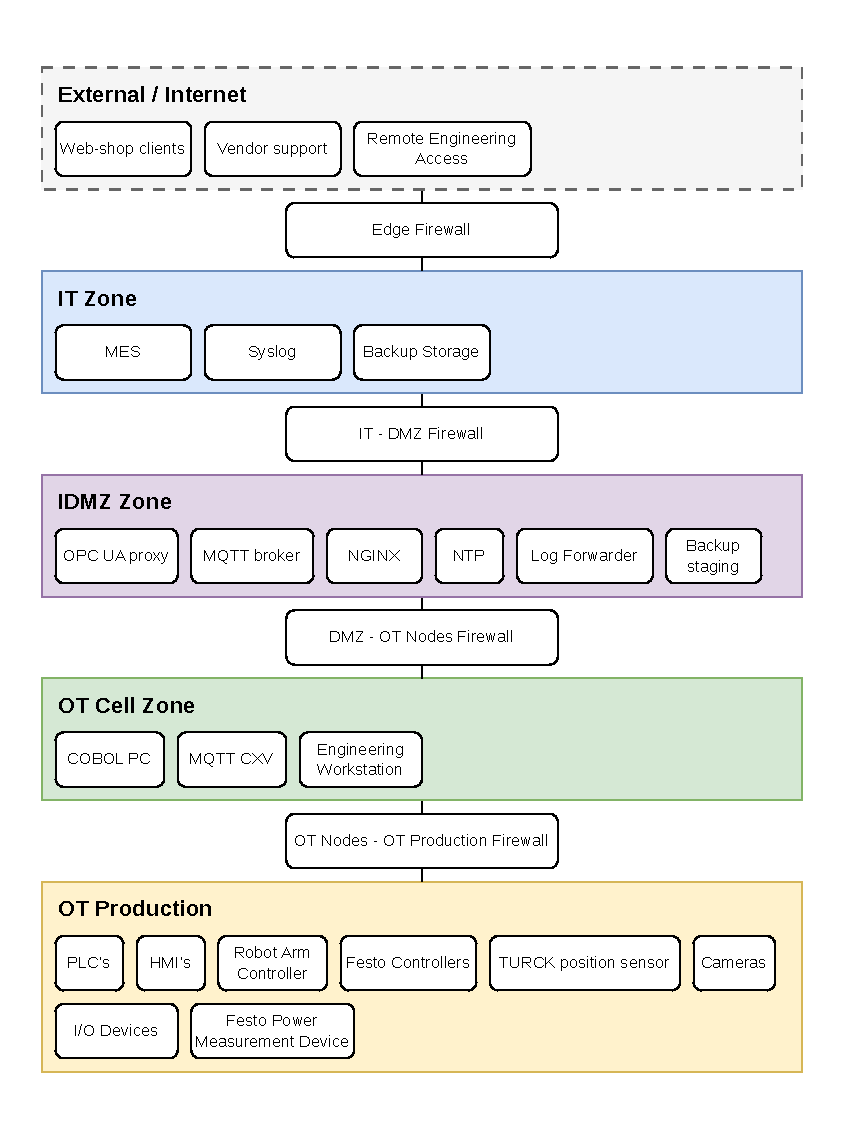
\includegraphics[width=1\textwidth]{img/logic_redesign.pdf}
    \caption{Zone \& Conduit Diagram}
\end{figure}

The current flat /18 network is replaced with a layered zone architecture based
on the IEC 62443 zone and conduit model. Each zone groups devices with similar
operational functions. All inter-zone traffic passes through a firewall and is
restricted to explicitly whitelisted traffic paths.

% 
\subsubsection{Logic Zones}
\textbf{IT Zone} \\ The IT Zone contains nodes handling business logic and
order management. It have no direct routed path to any OT device - all IT to OT
traffic goes through the IDMZ.

\textbf{IDMZ} \\ The IDMZ acts as a buffer between IT and OT devices. No
connecection is allowed to pass from the IT to OT and vice versa. Every traffic
exchange terminates inside IDMZ, and its re-innitiated to the other side. This
solution implements IEC 62443-3-3 SR 5.1 principle.

\textbf{OT Cell Zone} \\ The OT Cell Zone Contains devices supporting
production, but not beeing part of the physical production process. The
Enigneering Workstation is placed in this logical zone, however, in physical
implementation, this node will be further isolated into separate VLAN.

\textbf{OT Production Zone} \\ The OT Production Zone contains devices beeing
part of the direct physical production process. Only inbound traffic allowed in
this zone are reads and writes from the proxy services, and S7comm+ from the
engineering workstation.

\subsubsection{New Nodes} 
\textbf{OPC UA proxy} \\ In the AS-IS architecture,
MES can directly connect to the PLC's OPC UA servers over the flat network. OPC
UA proxy node aggregates all PLC's OPC UA servers traffic into single endpoint
inside IDMZ. The MES connects only to proxy, that is also responsible for
enforcing rules on what nodes are readable and writable from the MES.
Furthermore, it logs all sessions. This solution satisfies IEC 62443-3-3 SR
3.2.

\textbf{Nginx} \\ In AS-IS architecture, MES can directly access unencrypted
HTTP services from the OT nodes. As stated in security requirements, all not
strictly required HTTP servers of OT devices will be disabled. However, for
required HTTP traffic (e.g PLC's alarm table <- MES) the Nginx node is
introduced in IDMZ. MES connects to the Nginx over HTTPS TLS 1.2, terminates
the connection, access the requested HTTP node server and forwards it to the
MES. Nginx enforces authentication, logging all requests and block requests for
services that should not be reached from IT zone.

\textbf{Dedicated MQTT broker} \\ In the AS-IS architecture MQTT CVX device
publish messages over a flat network to the MES. MQTT broker node placed in
IDMZ, aggregates MQTT traffic from the CVX device using TLS 1.2 encryption, and
it restrict inbound traffic to publish messages only. MES is subscribes to the
MQTT broker, preventing direct communication between OT node and IT node. This
solution satisfies IEC 62443-3-3 SR 1.1 and SR 3.1.

\textbf{Engineering Workstation} \\ In the AS-IS architecture, TIA Portal is
run on the same PC as MES service - part of IT and reachable over flat network.
A dedicated Engineering Workstation is placed in the OT Cell Zone (physically
on separate VLAN). This workstation purpose is to program and configure PLC's
and HMI's with separation from IT nodes. Traffic is restricted only to TCP 102
on PLC's and HMI's. This enforces least-privilage and IEC 62443-2-1 §4.3.3.

\textbf{Syslog} \\ In the AS-IS architecture, there is no centralized logging
system implemented. Syslog node collects all logs from the firewalls, managed
switches, OPC UA and HTTP proxy, and MQTT broker. This provides post-attack
analysis and satisfies IEC 62443-3-3 SR 6.1 and NIS2 Article 21(2)(f).
\textbf{Backup} \\ In AS-IS architecture, there is no documented backup
procedure. The backup node recieves configuration backups from the Engineering
Workstation after every change and daily database backups from the MES. It is
placed on separate VLAN inside IT zone, separated from indbound traffic from
OT. Satisfies IEC 62443-2-1 §4.3.4 and ISO/IEC 27001 A.12.3.

\subsubsection{Firewalls} 
This section only describres briefly the high-level
purpose of the firewall nodes. Further specification on permitted conduits is
described in ~\ref{sec:secreq}

\textbf{Edge Firewall} \\ Terminates all VPN tunnels from remote engineers and
vendor support, enforces MFA before any traffic enters the IT zone, and blocks
all unsolicited inbound connections from the internet. Default-deny on all
inbound. Satisfies IEC 62443-2-1 §4.3.3.6 and NIS2 Article 21(2)(i).

\textbf{IT - DMZ Firewall} \\ Controls all traffic between the IT zone and the
IDMZ. 

\textbf{DMZ - OT Cell Firewall} \\ Controls traffic between the IDMZ and the OT
cell zone. 

\textbf{OT Cell - OT Production Firewall} \\ Controls traffic between the OT
cell zone and the six station VLANs. OPC UA proxy connections arrive from the
IDMZ side, not the cell zone side, so they do not pass this firewall. Profinet
never crosses this boundary — it remains Layer 2 within each station. All other
traffic denied. Satisfies IEC 62443-3-3 SR 5.1 and the least privilege
principle.

%% TOBE IMPLEMENTATION
\subsection{Network Implementation}\label{tobeimpl}
The Network Implementation diagram is appended to the report for better
visibility.
\begin{figure}[H]
    \centering
    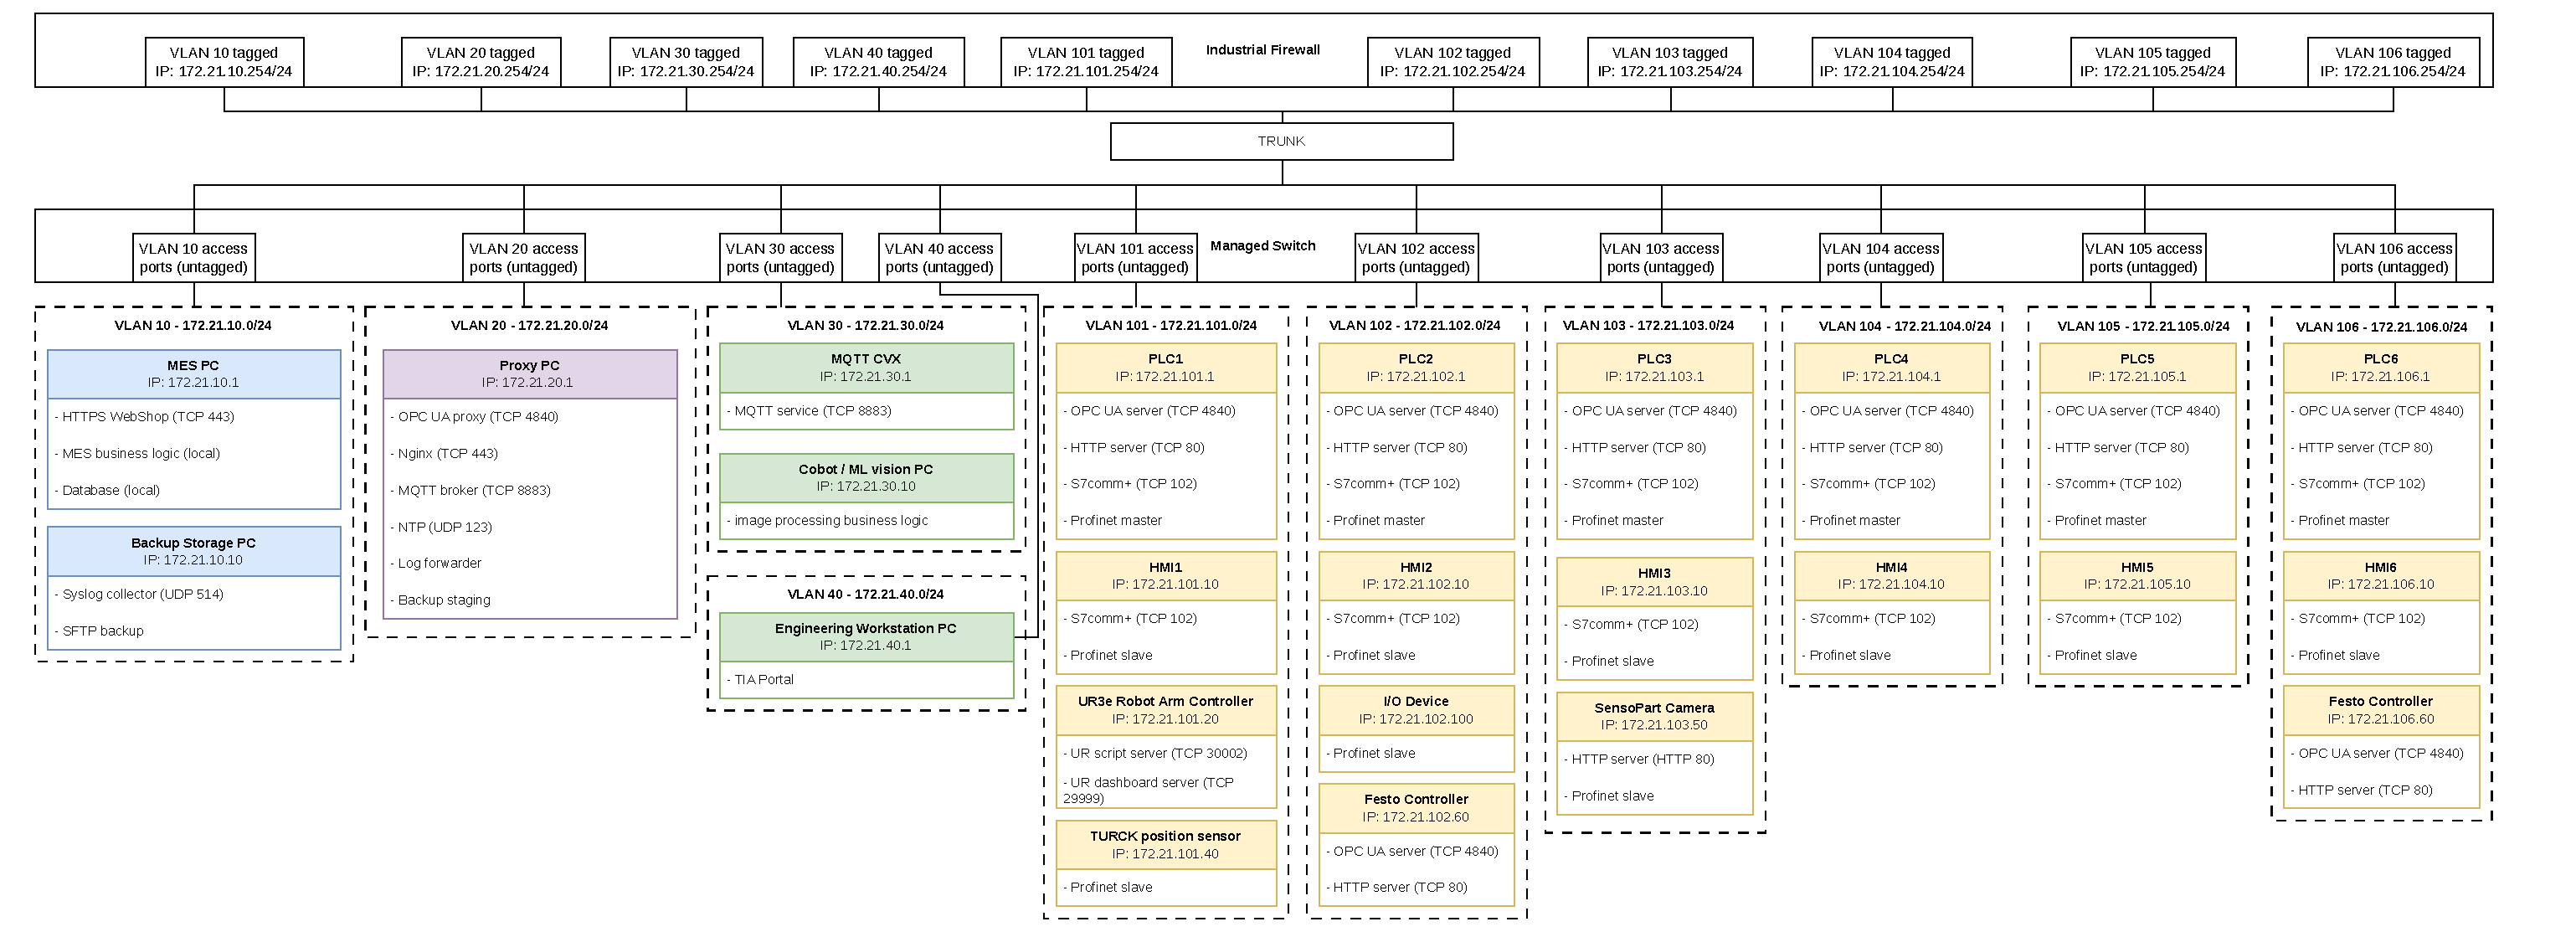
\includegraphics[width=1\textwidth]{img/redesign_iml.pdf}
    \caption{Network Implementation}
\end{figure}

\subsubsection{VLAN Segmentation \& Restricted Routing}
The redesigned factory network is implemented using VLAN-based segmentation on
managed industrial switches. Each security zone is assigned a dedicated VLAN
and IP subnet. Inter-VLAN communication is not performed by the switch itself
but is routed through a central industrial firewall. The firewall has one
tagged VLAN port for each VLAN - which is a default gateway for each node
withing that VLAN. The firewall enforces security policies between zones. A
VLAN trunk connection between the firewall and the managed switch transports
traffic for all security zones while preserving logical separation through IEEE
802.1Q VLAN tagging. \\ Because the switch never bridges VLANs, the only path
between any two zones is through the firewall. The firewall applies a
default-deny policy: traffic between VLANs is dropped unless a rule explicitly
permits it. Traffic within a VLAN (for example PLC-to-HMI Profinet inside one
station) is switched locally and never reaches the firewall. Profinet RT
traffic is Layer 2 only and is confined to its station VLAN; it is never routed
across the firewall. This realises the four logical firewall boundaries (Edge,
IT–IDMZ, IDMZ–OT Cell, OT Cell–OT Production) on a single physical firewall,
where each boundary corresponds to a rule set between the relevant VLAN
interfaces. It satisfies IEC 62443-3-3 SR 5.1 (Restricted Data Flow) and SR 5.2
(Zone Boundary Protection).

\renewcommand{\arraystretch}{1.3} % 30% more row height
\begin{tabularx}{\textwidth}{>{\bfseries}p{2.5cm} X X}
    VLAN & \textbf{Zone} & \textbf{Nodes} \vspace{0.5em}\\
\toprule
    10 & IT & MES PC, Data Storage PC \\
    20 & IDMZ & Proxy PC\\
    30 & OT Cell & COBOL PC, MQTT CVX \\
    40 & OT Cell - Engineering & Engineering Workstation  \\
    101 & OT Prod - Station 1 & PLC1, HMI1, UR3e Robot Arm Controller, TURCK position sensor \\
    102 & OT Prod - Station 2 & PLC2, HMI2, I/O device, Festo Controller \\
    103 & OT Prod - Station 3 & PLC3, HMI3, SensoPart Camera \\
    104 & OT Prod - Station 4 & PLC4, HMI4 \\
    105 & OT Prod - Station 5 & PLC5, HMI5 \\
    106 & OT Prod - Station 6 & PLC6, HMI6, Festo controller \\
\end{tabularx}

\section{Hardware \& Configuration Proposal}
\subsection{Protocol Hardening}
The redesign (see chapter~\ref{tobeimpl}) controls where each protocol may flow. This
chapter defines how each protocol is secured on the device and conduit level.

\subsubsection{Profinet}
Profinet has no authentication or encryption features, so it cannot be hardened
at the protocol level. Instead it is secured by isolation.
\begin{itemize}

    \item Layer 2 only - Profinet stays inside each OT Production station (VLAN
        101 - 106). It is never routed, and never crosses through firewall.
        Even if routing would be executed (through the attack) router would
        drop the communication.

    \item No inter-station Profinet communication - Each PLC talks Profinet
        (with I/O, HMI) only within own VLAN.

    \item DCP Set disabled - desible DCP Set through TIA Portal for devices
        that support this feature. This prevents rename/reconfigure attacks
        through DCP.

\end{itemize}

\subsubsection{OPC UA}

OPC UA is the only routed OT data protocol. Hardening is specified in SR-03.
TODO chapter reference)

\begin{itemize}

    \item Security mode Sign\&Encrypt - Security policy Basic256Sha256. Mode
        'none' is disabled on all PLC and Festo Controllers servers.

    \item Certificate authentication - Clients (OPC UA proxy, Cobot/MLvisionPC)
        authenticate with application certificates. Annonymous and
        username/password sessions are disabled.

    \item Scoped access - The Cobot/MLvisionPC can reach only PLC2 on Station
        2, and no other PLC's.

\end{itemize}

\subsubsection{MQTT}

MQTT is used by the Festo CXV device for telemetry. It's hardening is specified
in SR-04 TODO Chapter reference

\begin{itemize}

    \item MQTT broker in IDMZ - The MQTT CXV device publishes only to a
        dedicated MQTT broker placed in IDMZ. IT nodes can only subscribe to
        the broker. No direct OT-IT MQTT path exists.

    \item TLS 1.2+ - TLS encryption enforced on all MQTT connections.

    \item Client certificates - MQTT CXV device must authenticate with
        certificate for publish connection to the broker. No annonymous
        connections allowed.

    \item Topic ACL's - THe MQTT CXV device may publish only to it's own
        topics. IT nodes (MES) cannot publish to the OT topics.

\end{itemize}

\subsubsection{HTTP/Web Interfaces}
Some OT devices need to expose plaintext HTTP web interfaces. Hardening is
specified in SR-05 TODO chapter reference

\begin{itemize}

    \item Disabled by default - All HTTP servers are disabled unless strictly
        needed for operational functionality.

    \item Reverse proxy - Where web access is needed (e.g. MES reading the PLC
        alarm table), the MES connects to the Nginx reverse proxy in the IDMZ
        over HTTPS/TLS 1.2+. Nginx terminates the connection, fetches the
        OT-side resource, and returns it. Plaintext HTTP stays inside the OT
        zone.

    \item Access restriction - Ngnix authenticate requests, logs them and
        blocks any OT server that should not be reached from IT zone. Firewall
        rules restrict web access to the Nginx TCP/IP port only.

\end{itemize}

\subsubsection{S7comm+ Engineering Access}
S7comm+ connection is used only for programming PLC's and HMI's. Hardening is
sepcified in SR-06 and SR-07 TODO chapter reference

\begin{itemize}

    \item Single source - S7comm+/TCP102 to any PLC or HMI is allowed only from
        the dedicated Engineering Workstation in VLAN40.

    \item Conduit controll - Engineering Worksation S7comm+ connection
        initialization passes through the firewall, enforcing restriction of
        Engineering Station to PLC's and HMI's only.

    \item User Authentication - PLC's and HMI's access requires individual
        login/password authentication with role separation (implemented in TIA
        portal).

\end{itemize}

\subsection{Hardware Proposal}\label{hardwareproposal}
This chapter lists the hardware required to implement the redesigned
architecture (Chapter 7). 

\subsubsection{Industrial Firewall}
\renewcommand{\arraystretch}{1.3} % 30% more row height
\begin{tabularx}{\textwidth}{>{\bfseries}p{2.5cm} X}
    \toprule
    Model & Fortinet FortiGate Rugged 70G \\
    \midrule
    Function & Central Layer 3 firewall and inter-VLAN router. All traffic
    between VLANs passes through it - under default-deny polict. Can perform
    stateful filtering and packet inspection of industrial protocols (S7comm+,
    OPC UA, MQTT, HTTP/S). Implements four logical firewalls (Edge, IT–IDMZ,
    IDMZ–OT Cell, OT Cell–OT Production) as separate rule sets between VLAN
    interfaces. \\
    \midrule
    Placement & Network core. Has one tagged VLAN interface (.254 gateway) per
    VLAN. Has single 802.1Q trunk to the managed switch. No VLAN is bridged on
    the switch, so the firewall is the only inter-VLAN path. \\
    \midrule
\end{tabularx}

\subsubsection{Managed Switch}
\renewcommand{\arraystretch}{1.3} % 30% more row height
\begin{tabularx}{\textwidth}{>{\bfseries}p{2.5cm} X}
    \toprule
    Model & Siemens SCALANCE XC-216  \\
    \midrule
    Function & VLAN-aware Layer 2 switching with IEEE 802.1Q tagging. Provides
    per-station access ports (untagged, one VLAN each) and the trunk uplink to
    the firewall. \\
    \midrule
    Placement & Replace the existing unmanaged SCALANCE XB008 switches at each
    station. Interconnected by 802.1Q trunks; one trunk reaches the firewall.
    \\
    \midrule
\end{tabularx}

\subsubsection{Engineering Station}
\renewcommand{\arraystretch}{1.3} % 30% more row height
\begin{tabularx}{\textwidth}{>{\bfseries}p{2.5cm} X}
    \toprule
    Model & Siemens SIMATIC IPC627E\\
    \midrule
    Function & Dedicated managed station running TIA Portal for PLC and HMI
    programming/configuration. Only host permitted S7comm+ to PLCs/HMIs.\\
    \midrule
    Placement & OT Cell zone, isolated in its own VLAN (40). Reaches OT
    Production only through the firewall on TCP 102.\\
    \midrule
\end{tabularx}

\subsubsection{IDMZ proxy server}
\renewcommand{\arraystretch}{1.3} % 30% more row height
\begin{tabularx}{\textwidth}{>{\bfseries}p{2.5cm} X}
    \toprule
    Model & Industrial rack server or SIMATIC IPC. Hardened Linux.\\
    \midrule
    Function & Hosts the IDMZ services — OPC UA proxy, Nginx reverse proxy,
    MQTT broker, NTP master, log forwarder, backup staging. \\
    \midrule
    Placement & Placed inside IDMZ zone - on VLAN20. \\
    \midrule
\end{tabularx}

\subsubsection{Syslog \& Backup Storage}
\renewcommand{\arraystretch}{1.3} % 30% more row height
\begin{tabularx}{\textwidth}{>{\bfseries}p{2.5cm} X}
    \toprule
    Model & Standard server, Linux OS. \\
    \midrule
    Function & Central Syslog collector for firewall, switches, proxies and
    broker; offline configuration backups (after every change) and daily MES
    database backups over SFTP.\\
    \midrule
    Placement & IT zone, VLAN10\\
    \midrule
\end{tabularx}

\subsection{Standards Alignment}\label{standardsalignment}
This section briefly describes each standard referenced in the report and lists
the design and implementation measures applied against it.

\subsubsection{IEC 62443}
A series of standards for security of Industrial Automation and Control Systems
(IACS). Part~1-1 defines the zone-and-conduit model; part~2-1 covers the
cybersecurity management system (asset inventory, access management, change
control, time and backup); part~3-3 defines system security requirements (SRs)
for authentication, data flow restriction, and monitoring.

\textit{Measures applied:}
\begin{itemize}[nosep]
  \item Zone \& conduit model (1-1): four zones (IT, IDMZ, OT Cell, OT
      Production) with all inter-zone traffic through firewall conduits (SR-01,
        TO-BE \S6).

    \item Restricted data flow / zone boundary protection (3-3 SR 5.1/5.2):
        VLAN segmentation routed through a single industrial firewall under
        default-deny; the IDMZ terminates and re-initiates all IT--OT
        exchanges.

    \item Authentication (3-3 SR 1.1--1.3): OPC UA Sign\&Encrypt with
        certificates; MQTT TLS with client certificates; HTTPS web access;
        individual PLC/HMI logins with role separation.

    \item Logging (3-3 SR 6.1/6.2): central Syslog from firewalls, switches,
        proxies, and broker; firewalls log denied traffic.

    \item CSMS (2-1): dedicated Engineering Workstation and controlled change
        access (\S4.3.3); single NTP source and backup/recovery (\S4.3.4); Edge
        Firewall with MFA for remote access (\S4.3.3.6).
\end{itemize}

\subsubsection{ISO/IEC 27001}
An information security management standard whose Annex~A controls are applied
here in an OT context: asset management (A.8.1), network segmentation (A.8.22),
network security (A.8.20), access control (A.9), logging (A.12.4), and backup
(A.12.3).

\textit{Measures applied:}
\begin{itemize}[nosep]
  \item Asset management (A.8.1): structured inventory; requirement to identify
      and document undocumented devices (F-04, F-15).

  \item Segmentation and network security (A.8.22, A.8.20): VLAN/firewall
      separation between all zones (SR-01, SR-02).

  \item Access control (A.9): role-based access with individual accounts
      (SR-06).

  \item Logging (A.12.4): centralised Syslog (SR-08).

  \item Backup (A.12.3): scheduled, offline backups with tested recovery
      (SR-10).
\end{itemize}

\subsubsection{NIS2 Directive}
An EU directive on cybersecurity risk management for essential and important
entities. Article~21 covers risk-management measures, including segmentation
and access control (21(2)(d)), time/backup (21(2)(c)), monitoring (21(2)(f)),
basic cyber hygiene (21(2)(h)), supply-chain security (21(2)(e)), and secure
remote access (21(2)(i)).

\textit{Measures applied:}
\begin{itemize}[nosep]
  \item Risk management / segmentation (Art.~21, 21(2)(d)): zoned network with
      controlled conduits (SR-01).

  \item Backup and time (21(2)(c)): single NTP source and backup/recovery
      (SR-09, SR-10).

  \item Monitoring (21(2)(f)): central logging (SR-08).

  \item Cyber hygiene (21(2)(h)): network admission control and MQTT/TLS
      hardening (F-08, SR-04).

  \item Secure remote access (21(2)(i)): Edge Firewall with VPN termination and
      MFA.

  \item Supply chain (21(2)(e)): firmware verification of multi-vendor devices
      (F-10, F-13).
\end{itemize}

\subsubsection{Defense-in-Depth}
The principle of multiple independent, layered controls so that no single
failure exposes the whole system.

\textit{Measures applied:} layered zones (IT, IDMZ, OT Cell, OT Production)
with a firewall at each boundary; per-protocol hardening on top of
segmentation; the IDMZ as an additional buffer that prevents direct IT--OT
paths; logging and backup as fallback/recovery layers.

\subsubsection{Least Privilege \& Zero Trust}
Least privilege grants each component only the access it needs; Zero Trust
grants no implicit trust based on network location.

\textit{Measures applied:} default-deny firewall with explicitly whitelisted
protocol routes (\S6.4); the Cobot/ML vision PC scoped to PLC2 only; S7comm+
permitted only from the Engineering Workstation in VLAN 40; OPC UA reachable
only via the IDMZ proxy; trust based on authenticated identity and certificates
rather than subnet membership.

\section{Discussion and Limitations}
\subsection{Limitations}\label{limitations}

\textbf{Hardware.} There is limited hardware in the lab to fully implement a
proper Purdue-model architecture. Several services (proxies, broker, logging,
backup) would have to run on the same machine, which creates a single point of
failure.

\textbf{Complexity.} The Festo Factory purpose is to provide an educational
setup for OT systems learning. A fully secured model would decrease learning
experience.
Added authentication, role and privilege management, and access
steps make the system harder to work with for learning.

\textbf{Maintenance.} A more complex setup needs ongoing maintenance. In
practice this would require one dedicated person, trained on this specific
system, to keep it running and up to date.

\subsection{Project Difficulties}
The network traffic captures used for the AS-IS analysis and inventory in this
report were taken while the FESTO Smart Factory was operated manually at the
lab, rather than running its full automated production cycle. We were unable to
get the plant running end-to-end during the sessions, which means some
communication flows are assumed from documentation and partial observation
rather than confirmed in live traffic.
For example:
\begin{itemize}
    \item \textbf{Robot arm motion sequences} — captured only for isolated test
        movements, not a complete pick-and-place cycle, so the full range of
        commands exchanged with the PLC may not be reflected in our
        Communications Mapping.
    \item \textbf{MES-triggered workflows} — webshop order processing and the
        resulting MES-to-PLC instructions could not be captured under realistic
        load, since we did not have a live order to trigger the flow during our
        session.
    \item \textbf{Camera HTTP visual stream} — the Cobot-ML PC pulls inspection
        images from the SensoPart camera over HTTP. Without a running inspection
        cycle we did not capture these requests during real operation, so the
        request rate and content are assumed.
\end{itemize}

The inventory and AS-IS architecture is based on the captures we did obtain,
plus vendor documentation and protocol specifications. A follow-up assessment
with the plant running a full production cycle would be needed to confirm the
communications map is complete and that no device or flow was missed.

\section{General Reflection}
Our access to the plant was time-boxed and shared with other groups.
This limited how often we could repeat captures or test different operating
states. This is normal in OT, since production systems are rarely free for
security testing. Our experience was a smaller version of the access
negotiation that real OT assessments require.

The project also showed the gap between an ideal Purdue-model architecture and
what is actually deployed. Some captured flows did not match the zone boundaries
we expected. This shaped our threat modelling and several security requirements
in Section~\ref{sec:secreq} (for example the firewall conduits in SR-01 and
SR-02). We see this as a useful result on its own: segmentation for a system
like this should start from observed traffic, not from an assumed architecture.
\end{document}
